\documentclass[border=1mm, tikz,dvipsnames]{standalone} 
\usepackage{tikz} 
\usetikzlibrary{decorations.pathreplacing, decorations.markings} 
\usetikzlibrary{calc} 
\usepackage{xcolor}

\def\empty{} 
\pgfkeys{utils/.cd,
	set if not empty/.code n args={3}{%
		\def\arg{#2}%
		\ifx\arg\empty%
		\pgfkeys{#1={#3}}%
		\else%
		\pgfkeys{#1={#2}}%
		\fi%
	},
	set if labelpos not empty/.code n args={2}{%
		\def\arg{#1}%
		\ifx\arg\empty%
	\else%
		\def\argo{#2}%
		\ifx\argo\empty%
		\pgfkeys{/tikz/label={#1}}%
		\else%
		\pgfkeys{/tikz/label={#2}:{#1}}%
		\fi%
		\fi%
	},
	set if arrowpos not empty/.code n args={3}{%
		\def\arg{#1}%
		\def\arstyle{#3}%
		\ifx\arstyle\empty%
		\def\arr{\arrow[>=stealth]{>}}
		\else%
		\def\arr{#3}
		\fi%
		\ifx\arg\empty%
		\pgfkeys{/pgf/decoration/mark={at position #2 with {\arr}}}%
		\else%
		\pgfkeys{/pgf/decoration/mark={at position #1 with {\arr}}}%
		\fi%
	},
}
\tikzset{
	nodes/.style n args={4}{
		draw ,circle,outer sep=0.7mm,
		/utils/set if not empty={/tikz/fill}{#1}{black},
		/utils/set if not empty={/tikz/minimum size}{#4}{5},
		/utils/set if labelpos not empty={#2}{#3},
		line width = 0.7pt
},
	arc/.style n args={3}{
		postaction={
			decorate,
			decoration={markings,
				/utils/set if arrowpos not empty={#1}{1}{}%
			}
		},
		/utils/set if not empty={/tikz/line width}{#2}{0.7pt},
		{#3}
	}
}

\begin{document}
 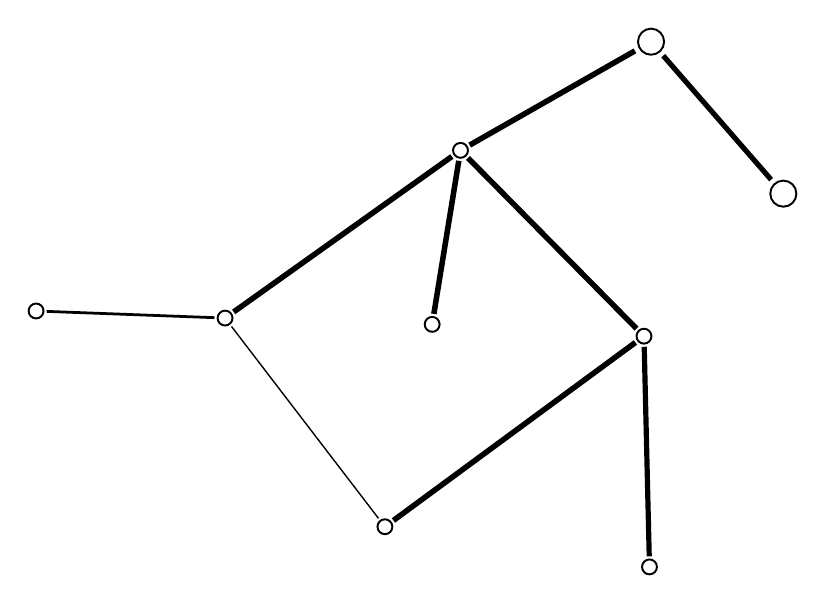
\begin{tikzpicture}[yscale=-1]
\node[scale = 0.5706885026737967, nodes={white}{}{}{}] (v0) at ( 7.165000000000003, 7.67 ) {};
\node[scale = 0.5706885026737967, nodes={white}{}{}{}] (v1) at ( 5.1350000000000025, 5.02 ) {};
\node[scale = 0.5706885026737967, nodes={white}{}{}{}] (v2) at ( 8.125000000000007, 2.8900000000000006 ) {};
\node[scale = 0.5706885026737967, nodes={white}{}{}{}] (v3) at ( 10.454999999999998, 5.249999999999995 ) {};
\node[scale = 0.5706885026737967, nodes={white}{}{}{}] (v4) at ( 7.765000000000002, 5.1 ) {};
\node[scale = 1, nodes={white}{}{}{}] (v5) at ( 10.545000000000002, 1.51 ) {};
\node[scale = 1, nodes={white}{}{}{}] (v6) at ( 12.224999999999998, 3.439999999999995 ) {};
\node[scale = 0.5706885026737967, nodes={white}{}{}{}] (v7) at ( 10.525000000000002, 8.18 ) {};
\node[scale = 0.5706885026737967, nodes={white}{}{}{}] (v8) at ( 2.735000000000002, 4.93 ) {};
\draw[line width = 0.5017546791443849] (v0) -- (v1);
\draw[line width = 1.999498663101604] (v1) -- (v2);
\draw[line width = 1.999498663101604] (v2) -- (v3);
\draw[line width = 1.999498663101604] (v3) -- (v0);
\draw[line width = 1.999498663101604] (v4) -- (v2);
\draw[line width = 1.999498663101604] (v2) -- (v5);
\draw[line width = 1.8741644385026734] (v5) -- (v6);
\draw[line width = 1.8741644385026734] (v3) -- (v7);
\draw[line width = 1] (v1) -- (v8);
\end{tikzpicture}
\end{document}